
\begin{figure*}[ht!]
\vspace{-10pt}
\begin{minipage}[c]{0.63\textwidth}
\centering
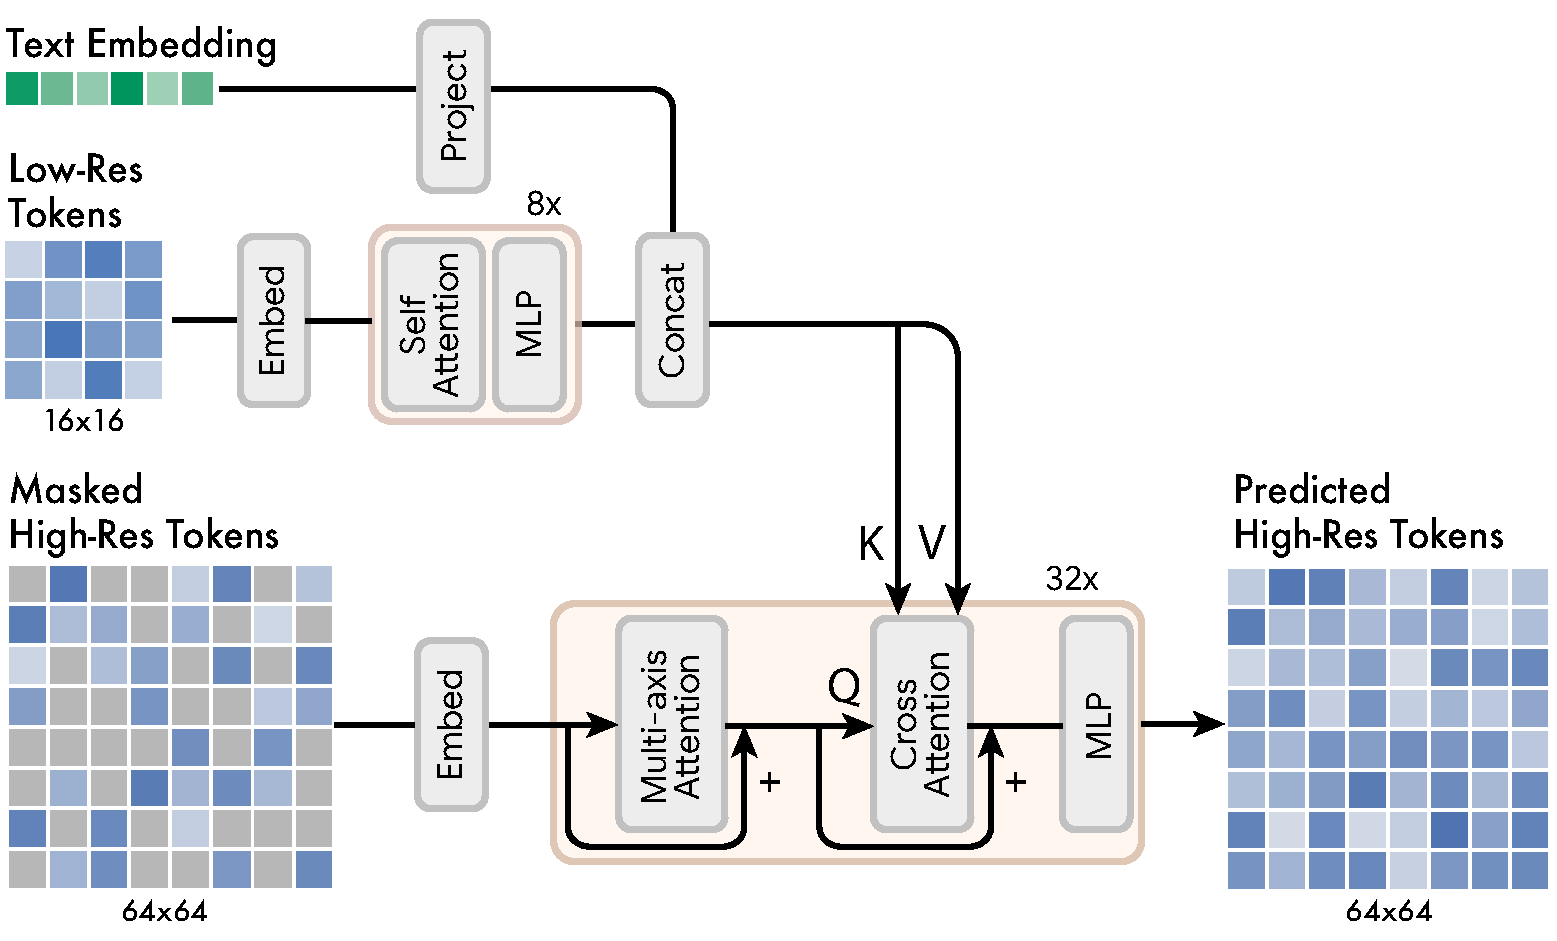
\includegraphics[width=\textwidth]{figs/superres_arch_fig}
%\caption{The architecture of the super-resolution model.}
\end{minipage} \hfill
%
\begin{minipage}[c]{0.34\textwidth}
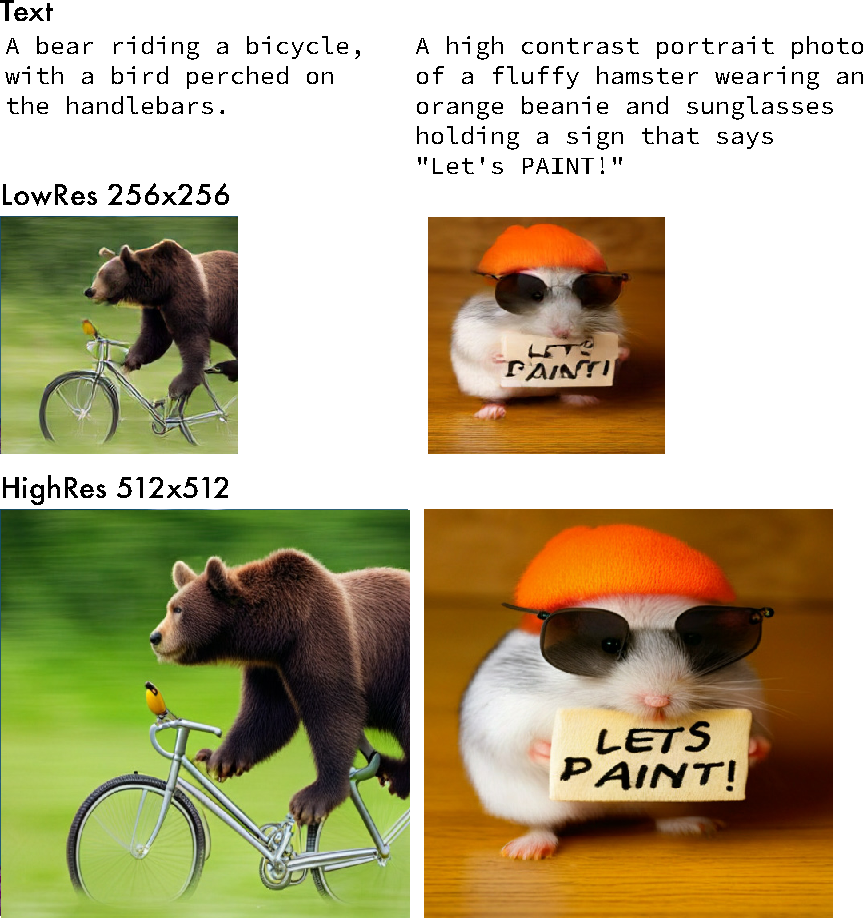
\includegraphics[width=\textwidth]{figs/superres_examples}
%\caption{Super-resolution examples.}
\end{minipage} 
\vspace{-5pt}
\caption{\small Super-resolution Model. On the left is shown the architecture of the super-resolution model. Low-resolution tokens are passed into a series of self-attention Transformer layers; and the resulting output embeddings are concatenated with text embeddings extracted from the conditioning text prompt. Following this, cross-attention is applied from these concatenated embeddings to the masked high-resolution tokens; the loss learns to predict these masked tokens conditioned on the low-resolution and text tokens. On the right are shown two examples of the improvement brought about by the super-resolution model.}

\label{fig:sr}
\end{figure*}